\section{Method}
While it relies on the same principles as in \cite{caldarelli2012network}, our proposed model is conceptually different : our ``products" are Wikipedia articles, which are not the basis for competitions but rather for cooperation. Editors enrich the articles together to make best articles. However, like countries, editors have limited capabilities and limited resources (e.g., time), which force them make choices on their contributions.

\begin{figure*}[!t]
\centering
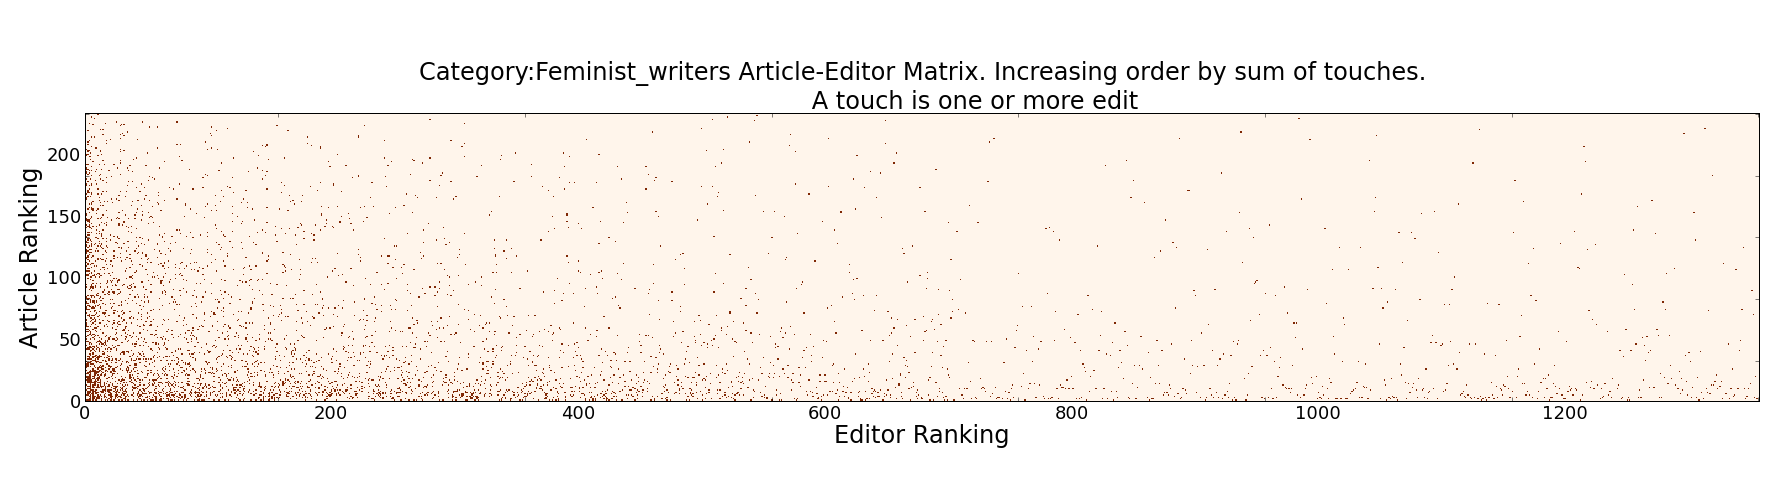
\includegraphics[width=2.0\columnwidth]{Figures/Category_Feminist_writerstriangle_matrix_corrected.png}.
\caption{Typical $\mathbf{M}$ matrix for a Wikipedia category (here, {\it Feminist Writers}) ordered on both dimensions by descending order of number of articles modified by an editor (horizontal axis) and of number editors who have modified an article (vertical axis). The structure of $\mathbf{M}$ is triangular and shows that some editors have a pervasive activity over articles, while most editors edit only a few. Similarly, some articles receive widespread attention by editors, while most articles are modified only by a few editors.}
\label{fig:triangle}
\end{figure*}


The matrix $\mathbf{M}$ shown in Figure \ref{fig:triangle_matrix} shows when an article has changed at some point by a given editor. The matrix is ordered on both dimensions by decreasing order of editors who have changed more articles (vertical axis) and by decreasing order of articles that have been changed by most editors (horizontal axis) for a category of Wikipedia articles (here Feminist Writers). Although it is a rough count, the matrix tells already about the experience of an editor in the given category, and the attention an article has gotten from editors, which is an implicit quality measure according to the second principle of peer-production : peer-review. This count is the zero order of the Article/Editor ranking algorithm, and thus the initiation step is given by 

\begin{equation}
\begin{cases}
 d_{e}^{(0)} = \sum_{a=1}^{N_{a}}\\
 u_{a}^{(0)} = \sum_{e=1}^{N_{N_{e}}}
\end{cases}
\end{equation}

Now, let's consider the second step :  if an article has been changed by editors who edited more articles, then the quality of the article should be higher. Similarly, if an editor has edited articles that have been edited by more editors, then the expertise of the editor should be higher (the only reason for making this claim is the collaborative nature of Wikipedia, and learning by imitation). Accordingly, the third step is the following : if an article has been changed by editors who edited more articles that have edited by more editors, then the quality of the article should be higher. Similarly, if an editor has edited articles that have been edited by more editors that have edited more articles, then the expertise of the editor should be higher. The algorithm goes on recursively, incorporating the quality (resp. expertise) information of the article (resp. editor) at the previous step. 

{\bf tell about the stochastic process here} \cite{caldarelli2012network}

{\bf say that it is a ranking algorithm. We care only about the ranking of articles and editors}

The algorithm at step $n$ then writes,

\begin{equation}
\begin{cases}
 w^{(n+1)}_c (\alpha,\beta) = \sum_{p=1}^{N_p}  \mathbf{G}_{cp}(\beta) \mathbf{w}^{(n)}_p (\alpha,\beta)\\
w^{(n+1)}_p (\alpha,\beta) = \sum_{c=1}^{N_c}  \mathbf{G}_{pc}(\beta) \mathbf{w}^{(n)}_c (\alpha,\beta)\\
\end{cases}
\end{equation}

where the Markov transition matrix $\mathbf{\hat{G}}$ is given by 

\begin{equation}
\begin{cases}
\mathbf{G}_{cp}(\beta) = \frac{\mathbf{M}_{cp} \mathbf{k}_{c}^{-\beta}}{\sum_{c' = 1}^{N_c} \mathbf{M}_{c'p} \mathbf{k}_{c'}^{-\beta}}\\
\mathbf{G}_{cp}(\beta) = \frac{\mathbf{M}_{cp} \mathbf{k}_{c}^{-\beta}}{\sum_{c' = 1}^{N_c} \mathbf{M}_{c'p} \mathbf{k}_{c'}^{-\beta}}\\
 \end{cases}
\end{equation}

The random walkers starting from editors jump to articles at odd steps, and back to editors from article at even steps. This is like walking between nodes that are connected by the adjacency matrix \ref{fig:triangle}.



A ranking-by-iteration plot shows how the ranking typically converges over iterations. As shown in Figure \ref{fig:convergence}, the algorithm converges in a non-trivial way, they can be reduced ergodic Markov chains \cite{Firm Grounds}. In the iterative solution we see how certain editors start low, but then climb in rankings. This means that they are editing few articles, but those articles are of higher quality. Likewise certain articles climb over iterations, they are edited by relatively few editors, but those editors are fitter.

With the following balance condition,

\begin{equation}
\mathbf{G}_{pc} \mathbf{w}^*_c = \mathbf{G}_{cp} \mathbf{w}^*_p
\end{equation}

An analytical solution can be found \cite{caldarelli}

\begin{equation}
\begin{cases}
 w^*_c = A(\sum^{N_p}_{p=1} M_{cp}k_p^{-\alpha})k_c^{-\beta} \\
w^*_p = B(\sum^{N_c}_{c=1} M_{cp}k_c^{-\beta})k_p^{-\alpha}
\end{cases}
\end{equation}

that we use onwards. Note that in the case $\alpha = \beta = 0$, the analytical solution is nothing else that the zero$^{th}$ of the reflection method \cite{}.

\begin{figure}[!t]
\centering
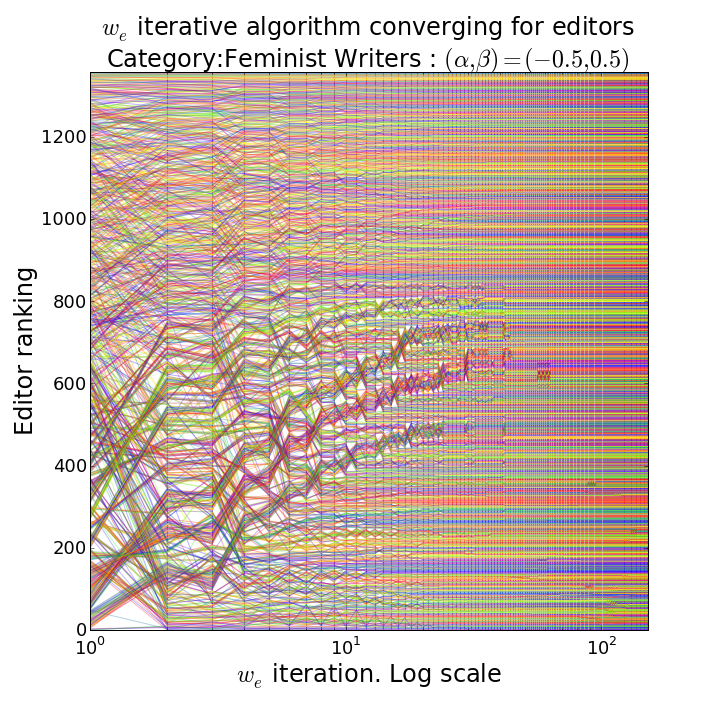
\includegraphics[width=0.9\columnwidth]{Figures/fem_editors_iter_converge.png}.
\caption{Convergence of $w_e$}
\label{fig:convergence}
\end{figure}

that we use onwards. Note that in the case $\alpha = \beta = 0$, the analytical solution is nothing else that the zero$^{th}$..

